%\clearpage
\section{Evaluation}
\label{sec:eval}
We now evaluate if \sysname meets our design goals
(\autoref{ssec:approach:goals}):

\begin{itemize}
  \item Can \sysname \emph{modularly} combine simulators into
    \emph{end-to-end} simulations?
    How do these simulations perform?
    (\autoref{ssec:eval:compsim})
    \item How \textit{efficient} is the \sysname synchronization mechanism?
        How does the overhead compare to prior approaches?
        (\autoref{ssec:eval:syncproto})
  \item Can \sysname enable \emph{faster} simulations by breaking down
    large simulators into smaller, parallel simulators?
    (\autoref{ssec:eval:decomp})
  \item How do larger \sysname simulations \emph{scale} on a single
    physical host and distributed across multiple physical hosts?
    (\autoref{ssec:eval:scalability})
  \item Does \sysname \emph{accurately} combine simulators?
    (\autoref{ssec:eval:accurate})
  \item Are \sysname simulations \emph{deterministic}?
    (\autoref{ssec:eval:deterministic})
\end{itemize}


\subsection{Experimental Setup}
Unless otherwise stated we use the following setup:
%
We run simulations on physical hosts with two 22-core Intel Xeon Gold 6152
processors at 2.10\,GHz with 187\,GB of memory, hyper-threading disabled, and
100\,Gbps Mellanox ConnectX-5 NICs.%
\footnote{The testbed  only affects simulation time and unsynchronized experiments.}
%
All simulated hosts have a single core and 8\,GB of memory, and each runs Ubuntu
18.04 with kernel 5.4.46 where we disabled unneeded features and drivers to
reduce boot time.
%
All device drivers and applications are unmodified.
%
For synchronized QEMU we set a clock frequency of 4GHz.
%
For gem5, we use \texttt{DDR4\_2400\_16x4} memory and the \texttt{TimingSimple}
CPU model, which simulates an in-order CPU with the timing memory protocol, and
configure cache sizes and latencies to match those of the testbed.
%
We set gem5 parameters (\eg, in-order CPU clock frequency of
8\,GHz~\footnote{Gem5 also supports an out-of-order CPU, but with
$4-6\times$ higher simulation time, so we use the TmingSimple CPU as a
compromise.}) to achieve the same effective instruction execution
performance as a representative physical testbed~\cite{kaufmann:tas},
for a Linux networking benchmark at 1.3\,cycles/inst = 0.43\,ns/inst.
%
Further, we set the PCIe latency, Ethernet link latency and
synchronization interval all to 500\,ns, network bandwidth to
10\,Gbps, and frequency for the Corundum RTL model to 250\,MHz.


%%%%%%%%%%%%%%%%%%%%%%%%%%%%%%%%%%%%%%%%%%%%%%%%%%%%%%%%%%%%%%%%%%%%%%%%%%%%%%%%
\subsection{\sysname is Modular}
\label{ssec:eval:compsim}
\paragraph{Navigating speed-accuracy trade-offs.}
We start by evaluating modular combinations of component simulators in
\sysname.
%
As a workload, we use the \texttt{netperf} TCP benchmark to run a 10s
throughput test (\texttt{TCP\_STREAM}) followed by a 10s latency test
(\texttt{TCP\_RR}) between two simulated hosts.
%
We focus on four configurations for common systems research
use-cases: debugging and performance evaluation of hardware and
software prototypes.
%
Debugging HW \& SW is most productive when fast and interactive,
while accurate performance is not the primary concern.
%
Here we combine QEMU with KVM for fast host simulation, our fast
switch model, and either the \texttt{i40e} NIC for SW testing or
Verilator with Corundum as a HW example.
%
Performance evaluation on the other hand requires accurate results, but it can
tolerate longer simulation times.
%
We use a detailed gem5 host simulator and ns-3 for SW performance evaluation,
while choosing a less detailed but time-synchronized QEMU simulator for
benchmarking our HW prototype.



\begin{table}%
\centering%
\begin{tabular}{lrrrr}%
    \toprule
    \textbf{Use-case} & \multicolumn{2}{c}{netperf} &
        \multicolumn{1}{c}{Sim.} \\
    Simulator Combination & T'put & Latency &
        \multicolumn{1}{c}{Time} \\
    \midrule

    \textbf{SW debugging} & 4.37\,G & 71\,$\mu$s & 00:00:32 \\
    \multicolumn{4}{l}{QEMU-kvm + behavioral i40e NIC + behavioral
      switch} \\[.3em]

    \textbf{SW perf. evaluation*} & 8.92\,G & 20\,$\mu$s & 12:49:46  \\
    \multicolumn{4}{l}{gem5 + behavioral i40e NIC + ns-3} \\[.3em]

    \textbf{HW debugging} & 81\,M & 3.4\,ms & 00:00:31 \\
    \multicolumn{4}{l}{QEMU-kvm + Corundum Verilog + behavioral
      switch} \\[.3em]

    \textbf{HW perf. evaluation*} & 6.55\,G & 32\,$\mu$s & 04:13:10 \\
    \multicolumn{4}{l}{QEMU-timing + Corundum Verilog + behavioral
      switch}\\
    \bottomrule\\
\end{tabular}%
\caption{\sysname configurations for different use-cases, with
    measured simulation time and application performance.
    Configurations with * are synchronized and deterministic, while
    the others are unsynchronized emulation.}%
\label{tab:modcombo}%
\vspace{-5mm}%
\end{table}

Our results in \autoref{tab:modcombo} confirm the expected trade-off between
simulation time and simulator detail: simulation times range from 31s to 18
hours.
%
The results show that, \sysname can effectively help navigate this trade-off by
only using detailed simulators when details matter for the use-case.
%
Even combining fast QEMU-kvm with an unsynchronized RTL simulation is
fast enough (31s) to test and debug the full system.
%
Modularity also allows us to late bind simulator choices, \eg if we
later realize that QEMU-timing is not sufficiently accurate, we can
replace it with gem5 without additional changes.


\paragraph{All combinations are functional.}
Besides these four configurations, we also evaluated the full cross-product of
simulator choices (\autoref{sec:impl}) and confirm \sysname supports all
combinations (subset of performance results in
\autoref{ssec:appendix:simcombos}).

\paragraph{\sysname interfaces are general.}
\sysname interfaces are generic and serve as narrow waists between
simulators.
%
To further demonstrate its generality, we extracted gem5's
\texttt{e1000} Intel NIC model, adapted it to \sysname's PCIe
interface without other modifications, and verified that it is
compatible with gem5 and QEMU.
%
To show that \sysname's PCIe interface generalizes beyond NICs, we
have adapted FEMU~\cite{li:femu}'s NVMe SSD model from their QEMU
fork into a separate simulator.
%
This simulator also works in combination with QEMU and gem5.


%%%%%%%%%%%%%%%%%%%%%%%%%%%%%%%%%%%%%%%%%%%%%%%%%%%%%%%%%%%%%%%%%%%%%%%%%%%%%%%%
\subsection{\sysname is Fast}
We now show \sysname does not significantly slow down simulators
through synchronization, and can even speed up simulations through
decomposition into parallel components.

\subsubsection{Synchronization}
\label{ssec:eval:syncproto}

\paragraph{Overhead.}
We measure synchronization overhead by comparing simulation time
for gem5 standalone and in \sysname.
%
The experiment does not use the network, but for synchronization, we
connect the gem5 to \texttt{i40e} NIC in \sysname and to our switch.
%
We first compare a low-event workload in gem5: executing
\texttt{sleep 10}.
%
The simulation takes 2.25\,min standalone and 2.91\,min in \sysname, a
30\% overhead.
%
This is the worst case -- gem5 is almost exclusively handling
\sysname synchronization events (every 500\,ns), as the CPU is mostly
halted.
%
For a high-event workload we use \texttt{dd} to read from
\texttt{/dev/urandom} to keep the CPU busy.
%
This simulation takes 100.26\,min standalone and 101.06\,min in
\sysname, a mere 0.8\% overhead.
%
\emph{\sysname incurs manageable synchronization overhead, and
does not significantly slow down already slow simulations.}

\paragraph{Comparison to dist-gem5.}
Next, we compare to dist-gem5~\cite{mohammad:distgem5} which
interconnects multiple gem5 instances and employs conventional
epoch-based global synchronization over TCP.
%
We configure 2 to 32 instances of gem5 that communicate pairwise using
iperf, through the \texttt{e1000} NIC in gem5 and a single switch.
%
For \sysname we use our gem5 Ethernet adapter to connect to our
switch model.
%
Our simulation time measurements in \autoref{fig:dist-gem} show that
\emph{\sysname is more efficient than dist-gem5, especially with
increasing scale}.
%
\sysname reduces simulation time by 27\% for 2 hosts, and by 74\% for 32 hosts.

\paragraph{Sensitivity to link latency.}
\sysname synchronization overhead is linked with the configured link
latency, which places a lower bound on sync message frequency.
%
We measure how link latency affects synchronization overhead, with
a pair of gem5 hosts running \texttt{netperf} for 1\,s of throughput
and latency measurements each, connected to \texttt{i40e} NICs and a
shared switch.
%
We vary the configured PCIe latency and sync interval, and report our
results in \autoref{fig:pcilat}.
%
While synchronization time does increase, \emph{lowering the link
latency by three orders of magnitude (from 1\,$\mu$s to 1\,ns) only
increases simulation time by 59\%}, demonstrating that \sysname can
effectively parallelize simulations across low-latency interconnects.


\begin{figure*}%
\centering%
\begin{minipage}{0.3\textwidth}%
\centering%
\begin{tikzpicture}[gnuplot]
%% generated with GNUPLOT 5.4p2 (Lua 5.4; terminal rev. Jun 2020, script rev. 114)
%% Tue 05 Jul 2022 09:49:52 PM CEST
\tikzset{every node/.append style={font={\fontsize{8.0pt}{9.6pt}\selectfont}}}
\path (0.000,0.000) rectangle (5.334,4.216);
\gpcolor{color=gp lt color border}
\gpsetlinetype{gp lt border}
\gpsetdashtype{gp dt solid}
\gpsetlinewidth{1.00}
\draw[gp path] (1.201,0.688)--(1.381,0.688);
\draw[gp path] (4.892,0.688)--(4.712,0.688);
\node[gp node right] at (1.201,0.688) {$0$};
\draw[gp path] (1.201,1.488)--(1.381,1.488);
\draw[gp path] (4.892,1.488)--(4.712,1.488);
\node[gp node right] at (1.201,1.488) {$500$};
\draw[gp path] (1.201,2.288)--(1.381,2.288);
\draw[gp path] (4.892,2.288)--(4.712,2.288);
\node[gp node right] at (1.201,2.288) {$1000$};
\draw[gp path] (1.201,3.089)--(1.381,3.089);
\draw[gp path] (4.892,3.089)--(4.712,3.089);
\node[gp node right] at (1.201,3.089) {$1500$};
\draw[gp path] (1.201,3.889)--(1.381,3.889);
\draw[gp path] (4.892,3.889)--(4.712,3.889);
\node[gp node right] at (1.201,3.889) {$2000$};
\node[gp node center] at (1.634,0.515) {2};
\node[gp node center] at (2.576,0.515) {8};
\node[gp node center] at (3.517,0.515) {16};
\node[gp node center] at (4.459,0.515) {32};
\draw[gp path] (1.201,3.969)--(1.201,0.688)--(4.892,0.688)--(4.892,3.969)--cycle;
\node[gp node center,rotate=-270] at (0.232,2.328) {Simulation Time [Min.]};
\node[gp node center] at (3.046,0.171) {Number of Simulated Hosts};
\node[gp node right] at (2.671,3.641) {dist-gem5};
\gpfill{rgb color={0.580,0.000,0.827}} (2.818,3.580)--(3.586,3.580)--(3.586,3.703)--(2.818,3.703)--cycle;
\gpcolor{rgb color={0.580,0.000,0.827}}
\draw[gp path] (2.818,3.580)--(3.586,3.580)--(3.586,3.702)--(2.818,3.702)--cycle;
\gpfill{rgb color={0.580,0.000,0.827}} (1.342,0.688)--(1.626,0.688)--(1.626,1.467)--(1.342,1.467)--cycle;
\draw[gp path] (1.342,0.688)--(1.342,1.466)--(1.625,1.466)--(1.625,0.688)--cycle;
\gpfill{rgb color={0.580,0.000,0.827}} (2.284,0.688)--(2.567,0.688)--(2.567,1.789)--(2.284,1.789)--cycle;
\draw[gp path] (2.284,0.688)--(2.284,1.788)--(2.566,1.788)--(2.566,0.688)--cycle;
\gpfill{rgb color={0.580,0.000,0.827}} (3.225,0.688)--(3.509,0.688)--(3.509,2.134)--(3.225,2.134)--cycle;
\draw[gp path] (3.225,0.688)--(3.225,2.133)--(3.508,2.133)--(3.508,0.688)--cycle;
\gpfill{rgb color={0.580,0.000,0.827}} (4.167,0.688)--(4.450,0.688)--(4.450,3.554)--(4.167,3.554)--cycle;
\draw[gp path] (4.167,0.688)--(4.167,3.553)--(4.449,3.553)--(4.449,0.688)--cycle;
\gpcolor{color=gp lt color border}
\node[gp node right] at (2.671,3.346) {\sysname};
\gpfill{rgb color={0.000,0.620,0.451}} (2.818,3.285)--(3.586,3.285)--(3.586,3.408)--(2.818,3.408)--cycle;
\gpcolor{rgb color={0.000,0.620,0.451}}
\draw[gp path] (2.818,3.285)--(3.586,3.285)--(3.586,3.407)--(2.818,3.407)--cycle;
\gpfill{rgb color={0.000,0.620,0.451}} (1.644,0.688)--(1.927,0.688)--(1.927,1.249)--(1.644,1.249)--cycle;
\draw[gp path] (1.644,0.688)--(1.644,1.248)--(1.926,1.248)--(1.926,0.688)--cycle;
\gpfill{rgb color={0.000,0.620,0.451}} (2.585,0.688)--(2.869,0.688)--(2.869,1.265)--(2.585,1.265)--cycle;
\draw[gp path] (2.585,0.688)--(2.585,1.264)--(2.868,1.264)--(2.868,0.688)--cycle;
\gpfill{rgb color={0.000,0.620,0.451}} (3.527,0.688)--(3.810,0.688)--(3.810,1.291)--(3.527,1.291)--cycle;
\draw[gp path] (3.527,0.688)--(3.527,1.290)--(3.809,1.290)--(3.809,0.688)--cycle;
\gpfill{rgb color={0.000,0.620,0.451}} (4.468,0.688)--(4.752,0.688)--(4.752,1.430)--(4.468,1.430)--cycle;
\draw[gp path] (4.468,0.688)--(4.468,1.429)--(4.751,1.429)--(4.751,0.688)--cycle;
\gpcolor{color=gp lt color border}
\node[gp node center] at (1.634,1.658) {-27\%};
\node[gp node center] at (2.576,1.980) {-47\%};
\node[gp node center] at (3.517,2.325) {-58\%};
\node[gp node center] at (4.459,3.745) {-74\%};
\draw[gp path] (1.201,3.969)--(1.201,0.688)--(4.892,0.688)--(4.892,3.969)--cycle;
%% coordinates of the plot area
\gpdefrectangularnode{gp plot 1}{\pgfpoint{1.201cm}{0.688cm}}{\pgfpoint{4.892cm}{3.969cm}}
\end{tikzpicture}
%% gnuplot variables
%
\caption{dist-gem5 vs. \sysname.}%
\label{fig:dist-gem}%
\end{minipage}%
\hfill%
\hfill%
\begin{minipage}{0.3\textwidth}%
\centering%
\begin{tikzpicture}[gnuplot]
%% generated with GNUPLOT 5.4p2 (Lua 5.4; terminal rev. Jun 2020, script rev. 114)
%% Tue 05 Jul 2022 09:49:52 PM CEST
\tikzset{every node/.append style={font={\fontsize{8.0pt}{9.6pt}\selectfont}}}
\path (0.000,0.000) rectangle (5.334,4.216);
\gpcolor{color=gp lt color border}
\gpsetlinetype{gp lt border}
\gpsetdashtype{gp dt solid}
\gpsetlinewidth{1.00}
\draw[gp path] (1.054,0.688)--(1.234,0.688);
\draw[gp path] (4.892,0.688)--(4.712,0.688);
\node[gp node right] at (1.054,0.688) {$0$};
\draw[gp path] (1.054,1.469)--(1.234,1.469);
\draw[gp path] (4.892,1.469)--(4.712,1.469);
\node[gp node right] at (1.054,1.469) {$50$};
\draw[gp path] (1.054,2.250)--(1.234,2.250);
\draw[gp path] (4.892,2.250)--(4.712,2.250);
\node[gp node right] at (1.054,2.250) {$100$};
\draw[gp path] (1.054,3.032)--(1.234,3.032);
\draw[gp path] (4.892,3.032)--(4.712,3.032);
\node[gp node right] at (1.054,3.032) {$150$};
\draw[gp path] (1.054,3.813)--(1.234,3.813);
\draw[gp path] (4.892,3.813)--(4.712,3.813);
\node[gp node right] at (1.054,3.813) {$200$};
\draw[gp path] (1.709,0.688)--(1.709,0.868);
\draw[gp path] (1.709,3.969)--(1.709,3.789);
\node[gp node center] at (1.709,0.515) {$5$};
\draw[gp path] (2.645,0.688)--(2.645,0.868);
\draw[gp path] (2.645,3.969)--(2.645,3.789);
\node[gp node center] at (2.645,0.515) {$10$};
\draw[gp path] (3.581,0.688)--(3.581,0.868);
\draw[gp path] (3.581,3.969)--(3.581,3.789);
\node[gp node center] at (3.581,0.515) {$15$};
\draw[gp path] (4.518,0.688)--(4.518,0.868);
\draw[gp path] (4.518,3.969)--(4.518,3.789);
\node[gp node center] at (4.518,0.515) {$20$};
\draw[gp path] (1.054,3.969)--(1.054,0.688)--(4.892,0.688)--(4.892,3.969)--cycle;
\node[gp node center,rotate=-270] at (0.232,2.328) {Simulation Time [Min.]};
\node[gp node center] at (2.973,0.171) {Number of Simulated Hosts};
\gpcolor{rgb color={0.580,0.000,0.827}}
\draw[gp path] (1.148,2.845)--(1.709,2.881)--(2.645,3.345)--(3.581,3.271)--(4.705,3.901);
\gpsetpointsize{4.00}
\gp3point{gp mark 1}{}{(1.148,2.845)}
\gp3point{gp mark 1}{}{(1.709,2.881)}
\gp3point{gp mark 1}{}{(2.645,3.345)}
\gp3point{gp mark 1}{}{(3.581,3.271)}
\gp3point{gp mark 1}{}{(4.705,3.901)}
\gpcolor{color=gp lt color border}
\draw[gp path] (1.054,3.969)--(1.054,0.688)--(4.892,0.688)--(4.892,3.969)--cycle;
%% coordinates of the plot area
\gpdefrectangularnode{gp plot 1}{\pgfpoint{1.054cm}{0.688cm}}{\pgfpoint{4.892cm}{3.969cm}}
\end{tikzpicture}
%% gnuplot variables
%
\caption{\sysname local scalability.}%
\label{fig:machines-scale}%
\end{minipage}%
\hfill%
\begin{minipage}{0.3\textwidth}%
\centering%
\begin{tikzpicture}[gnuplot]
%% generated with GNUPLOT 5.4p2 (Lua 5.4; terminal rev. Jun 2020, script rev. 114)
%% Tue 05 Jul 2022 09:49:52 PM CEST
\tikzset{every node/.append style={font={\fontsize{8.0pt}{9.6pt}\selectfont}}}
\path (0.000,0.000) rectangle (5.334,4.216);
\gpcolor{color=gp lt color border}
\gpsetlinetype{gp lt border}
\gpsetdashtype{gp dt solid}
\gpsetlinewidth{1.00}
\draw[gp path] (1.201,0.688)--(1.381,0.688);
\draw[gp path] (4.892,0.688)--(4.712,0.688);
\node[gp node right] at (1.201,0.688) {$0$};
\draw[gp path] (1.201,1.285)--(1.381,1.285);
\draw[gp path] (4.892,1.285)--(4.712,1.285);
\node[gp node right] at (1.201,1.285) {$200$};
\draw[gp path] (1.201,1.881)--(1.381,1.881);
\draw[gp path] (4.892,1.881)--(4.712,1.881);
\node[gp node right] at (1.201,1.881) {$400$};
\draw[gp path] (1.201,2.478)--(1.381,2.478);
\draw[gp path] (4.892,2.478)--(4.712,2.478);
\node[gp node right] at (1.201,2.478) {$600$};
\draw[gp path] (1.201,3.074)--(1.381,3.074);
\draw[gp path] (4.892,3.074)--(4.712,3.074);
\node[gp node right] at (1.201,3.074) {$800$};
\draw[gp path] (1.201,3.671)--(1.381,3.671);
\draw[gp path] (4.892,3.671)--(4.712,3.671);
\node[gp node right] at (1.201,3.671) {$1000$};
\draw[gp path] (1.201,0.688)--(1.201,0.868);
\node[gp node center] at (1.201,0.515) {$0$};
\draw[gp path] (1.911,0.688)--(1.911,0.868);
\node[gp node center] at (1.911,0.515) {$200$};
\draw[gp path] (2.621,0.688)--(2.621,0.868);
\node[gp node center] at (2.621,0.515) {$400$};
\draw[gp path] (3.330,0.688)--(3.330,0.868);
\node[gp node center] at (3.330,0.515) {$600$};
\draw[gp path] (4.040,0.688)--(4.040,0.868);
\node[gp node center] at (4.040,0.515) {$800$};
\draw[gp path] (4.750,0.688)--(4.750,0.868);
\node[gp node center] at (4.750,0.515) {$1000$};
\draw[gp path] (1.201,3.969)--(1.201,0.688)--(4.892,0.688)--(4.892,3.969)--cycle;
\node[gp node center,rotate=-270] at (0.232,2.328) {Simulation Time [Min.]};
\node[gp node center] at (3.046,0.171) {Number of Simulated Hosts};
\node[gp node right] at (3.683,2.475) {gem5};
\gpcolor{rgb color={0.580,0.000,0.827}}
\draw[gp path] (3.830,2.475)--(4.598,2.475);
\draw[gp path] (1.343,3.462)--(4.750,3.845);
\gpsetpointsize{4.00}
\gp3point{gp mark 1}{}{(1.343,3.462)}
\gp3point{gp mark 1}{}{(4.750,3.845)}
\gp3point{gp mark 1}{}{(4.214,2.475)}
\gpcolor{color=gp lt color border}
\node[gp node right] at (3.683,2.180) {QEMU-timing};
\gpcolor{rgb color={0.000,0.620,0.451}}
\draw[gp path] (3.830,2.180)--(4.598,2.180);
\draw[gp path] (1.343,1.082)--(1.911,1.243)--(2.621,1.386)--(3.330,1.493)--(4.750,1.690);
\gp3point{gp mark 2}{}{(1.343,1.082)}
\gp3point{gp mark 2}{}{(1.911,1.243)}
\gp3point{gp mark 2}{}{(2.621,1.386)}
\gp3point{gp mark 2}{}{(3.330,1.493)}
\gp3point{gp mark 2}{}{(4.750,1.690)}
\gp3point{gp mark 2}{}{(4.214,2.180)}
\gpcolor{color=gp lt color border}
\draw[gp path] (1.201,3.969)--(1.201,0.688)--(4.892,0.688)--(4.892,3.969)--cycle;
%% coordinates of the plot area
\gpdefrectangularnode{gp plot 1}{\pgfpoint{1.201cm}{0.688cm}}{\pgfpoint{4.892cm}{3.969cm}}
\end{tikzpicture}
%% gnuplot variables
%
\caption{Distributed scalability.}%
\label{fig:large-scale}%
\end{minipage}%
\Description{Three sub-figures (6, 7, and 8) with graphs showing simulation
  time on the y-axis.

  The first graph (figure 6) shows simulation time of
  dist-gem5 compared to \sysname for varying number of simulated hosts on the
  x-axis from 2 to 32. dist-gem5 is slower across the board and shows
  exponentially increasing simulation time, while for \sysname it only slowly
  increases. For two hosts \sysname is 27\% faster at around 360 min, and 74\%
  faster for 32 at close to 450 min.

  The second figure shows a line graph for gem5 in \sysname as the number of
  hosts increases from 2 to 21. Bettween 2 and 5 the line is flat at 140
  minutes, increasing to about 170 for 10 and 15, finally increasing to around
  210 for 21 simulated hosts.

  The third figure is another line graph, comparing gem5 and QEMU-timing for a
  distributed experiment. For QEMU-timing simulation time increases
  approximately linearly from 130 min with 40 hosts to about 330 with
  1000 hosts. With gem-5 it increases from 930 min with 40 hosts to
  about 1060 with 1000 hosts.}%
\end{figure*}


\subsubsection{Decomposition for Parallelism}
\label{ssec:eval:decomp}
%
\paragraph{Extracting NIC from gem5.}
When connecting synchronized simulators, the best \sysname can achieve
is to not slow them down beyond the slowest component simulator.
%
However, \sysname enables developers to decompose monolithic
simulators into connected components (\autoref{ssec:eval:compsim})
running in parallel, thereby accelerating simulation.
%
We evaluate this by comparing two gem5 configurations in \sysname:
first, gem5 with the built-in \texttt{e1000} NIC connected via our
Ethernet adapter, and second, gem5 connected to our \texttt{i40e} NIC
model through the PCIe interface.
%
In both cases we run a pair of hosts connected to our switch model.
%
The first configuration takes 350 minutes, while the second only takes 138
minutes: \emph{Parallelism from the external NIC simulator reduces simulation
time by 60\%}.

\paragraph{Network simulator as scalability bottleneck.}
Network simulators are potential scalability bottlenecks in \sysname,
as they often connect many NICs, while hosts and NICs typically only connect
one and two peers, respectively.
%
To demonstrate this bottleneck, we develop a packet generator as a dummy NIC
that implements the \sysname Ethernet interface and the synchronization
mechanism.
%
The dummy NIC simply injects packets at a configured rate.
%
We now measure simulation time for 2 and 32 dummy NICs connected to
one switch for 1 second of virtual time.
%
First we set the packet rate to 0 (to only measure synchronization overhead) and
measure an increase from 2.6\,s to 17.6\,s of simulation time.
%
Next, we set the packet rate to 100\,Gbps on each NIC, and measure the
simulation time increases from 12.6\,s to 211.6\,s.
%
This experiment confirms that \emph{a single network simulator can become a
bottleneck for fast simulations}.
%
We have so far not observed this outside of this microbenchmark.

\paragraph{Parallelizing network simulation.}
To address this bottleneck in \sysname, we can decompose the network into
multiple network simulators carved up at natural boundaries (\eg switches or
groups thereof).
%
We demonstrate this by modifying the microbenchmark to divide the 32
hosts to 4 ``ToR'' switches, connected through a fifth ``core''
switch.
%
With this configuration, the simulation time for packet rate 0 is 9.6\,s down by
45\% compared to the single switch setup, and 96.8\,s at 100\,Gbps packet rate,
a 53\% reduction.
%
\emph{Decomposing network simulators, therefore, can effectively reduce
simulation time at scale.}


%%%%%%%%%%%%%%%%%%%%%%%%%%%%%%%%%%%%%%%%%%%%%%%%%%%%%%%%%%%%%%%%%%%%%%%%%%%%%%%%
\subsection{\sysname is Scalable}
\label{ssec:eval:scalability}
We now evaluate scalability for local and distributed simulations.

\subsubsection{Scaling Up}\hfill\\
First, we measure simulation time as we vary the number of simulated
gem5 hosts and \texttt{i40e} NICs connected to a single switch,
running on a single physical host.
%
We set up one server and a variable number of client hosts, running
the same UDP iperf benchmark.
%\jialin{is it iperf or netperf?}
%
To avoid overloading the server, we fix the aggregate throughput to
1\,Gbps.
%
The results in \autoref{fig:machines-scale} show the simulation time
increases with the number of clients, from 138\,min with 2
hosts to 205\,min with 21 hosts (48\% increase).

Surprisingly, the longer simulation time is \emph{not} caused by scalability
bottlenecks in \sysname synchronization.
%
Instead, we discovered that this increase is due to thermal
throttling of our host CPU slowing down all cores as more active.
%
To confirm this, we run multiple independent instances of the
1-client experiment and measure how this affects simulation time.
%
When running 4 independent instances of the 2-host simulations (5
cores each), using a total of 20 cores in the same NUMA node, the
simulation takes 171\,min.
%
This matches the runtime of the 10-host simulation above, which uses
21 cores in total.
%
We conclude that \emph{\sysname scales at least to the moderate
cluster sizes typical for many of our evaluations}.


\begin{figure*}%
\centering%
\begin{minipage}{0.28\textwidth}%
\centering%
\begin{tikzpicture}[gnuplot]
%% generated with GNUPLOT 5.4p2 (Lua 5.4; terminal rev. Jun 2020, script rev. 114)
%% Tue 05 Jul 2022 09:49:52 PM CEST
\tikzset{every node/.append style={font={\fontsize{8.0pt}{9.6pt}\selectfont}}}
\path (0.000,0.000) rectangle (5.334,4.216);
\gpcolor{color=gp lt color border}
\gpsetlinetype{gp lt border}
\gpsetdashtype{gp dt solid}
\gpsetlinewidth{1.00}
\draw[gp path] (1.054,0.688)--(1.234,0.688);
\draw[gp path] (4.892,0.688)--(4.712,0.688);
\node[gp node right] at (1.054,0.688) {$0$};
\draw[gp path] (1.054,1.235)--(1.234,1.235);
\draw[gp path] (4.892,1.235)--(4.712,1.235);
\node[gp node right] at (1.054,1.235) {$20$};
\draw[gp path] (1.054,1.782)--(1.234,1.782);
\draw[gp path] (4.892,1.782)--(4.712,1.782);
\node[gp node right] at (1.054,1.782) {$40$};
\draw[gp path] (1.054,2.329)--(1.234,2.329);
\draw[gp path] (4.892,2.329)--(4.712,2.329);
\node[gp node right] at (1.054,2.329) {$60$};
\draw[gp path] (1.054,2.875)--(1.234,2.875);
\draw[gp path] (4.892,2.875)--(4.712,2.875);
\node[gp node right] at (1.054,2.875) {$80$};
\draw[gp path] (1.054,3.422)--(1.234,3.422);
\draw[gp path] (4.892,3.422)--(4.712,3.422);
\node[gp node right] at (1.054,3.422) {$100$};
\draw[gp path] (1.054,3.969)--(1.234,3.969);
\draw[gp path] (4.892,3.969)--(4.712,3.969);
\node[gp node right] at (1.054,3.969) {$120$};
\draw[gp path] (1.822,0.688)--(1.822,0.868);
\node[gp node center] at (1.822,0.442) {1};
\draw[gp path] (2.589,0.688)--(2.589,0.868);
\node[gp node center] at (2.589,0.442) {10};
\draw[gp path] (3.357,0.688)--(3.357,0.868);
\node[gp node center] at (3.357,0.442) {100};
\draw[gp path] (4.124,0.688)--(4.124,0.868);
\node[gp node center] at (4.124,0.442) {1000};
\draw[gp path] (1.054,3.969)--(1.054,0.688)--(4.892,0.688)--(4.892,3.969)--cycle;
\node[gp node center,rotate=-270] at (0.232,2.328) {Simulation Time [Min.]};
\node[gp node center] at (2.973,0.171) {PCIe latency [ns]};
\gpfill{rgb color={0.416,0.318,0.639}} (1.630,0.688)--(2.015,0.688)--(2.015,3.779)--(1.630,3.779)--cycle;
\gpcolor{rgb color={0.416,0.318,0.639}}
\gpsetlinewidth{2.00}
\draw[gp path] (1.630,0.688)--(1.630,3.778)--(2.014,3.778)--(2.014,0.688)--cycle;
\gpfill{rgb color={0.416,0.318,0.639}} (2.397,0.688)--(2.782,0.688)--(2.782,3.259)--(2.397,3.259)--cycle;
\draw[gp path] (2.397,0.688)--(2.397,3.258)--(2.781,3.258)--(2.781,0.688)--cycle;
\gpfill{rgb color={0.416,0.318,0.639}} (3.165,0.688)--(3.550,0.688)--(3.550,3.314)--(3.165,3.314)--cycle;
\draw[gp path] (3.165,0.688)--(3.165,3.313)--(3.549,3.313)--(3.549,0.688)--cycle;
\gpfill{rgb color={0.416,0.318,0.639}} (3.933,0.688)--(4.317,0.688)--(4.317,2.630)--(3.933,2.630)--cycle;
\draw[gp path] (3.933,0.688)--(3.933,2.629)--(4.316,2.629)--(4.316,0.688)--cycle;
\gpcolor{color=gp lt color border}
\gpsetlinewidth{1.00}
\draw[gp path] (1.822,3.746)--(1.822,3.809);
\draw[gp path] (1.732,3.746)--(1.912,3.746);
\draw[gp path] (1.732,3.809)--(1.912,3.809);
\draw[gp path] (2.589,3.234)--(2.589,3.282);
\draw[gp path] (2.499,3.234)--(2.679,3.234);
\draw[gp path] (2.499,3.282)--(2.679,3.282);
\draw[gp path] (3.357,3.299)--(3.357,3.327);
\draw[gp path] (3.267,3.299)--(3.447,3.299);
\draw[gp path] (3.267,3.327)--(3.447,3.327);
\draw[gp path] (4.124,2.620)--(4.124,2.638);
\draw[gp path] (4.034,2.620)--(4.214,2.620);
\draw[gp path] (4.034,2.638)--(4.214,2.638);
\draw[gp path] (1.054,3.969)--(1.054,0.688)--(4.892,0.688)--(4.892,3.969)--cycle;
%% coordinates of the plot area
\gpdefrectangularnode{gp plot 1}{\pgfpoint{1.054cm}{0.688cm}}{\pgfpoint{4.892cm}{3.969cm}}
\end{tikzpicture}
%% gnuplot variables
%
\caption{Sensitivity of \sysname simulation time to link latency.}%
\label{fig:pcilat}%
\end{minipage}%
\hfill%
\begin{minipage}{0.45\textwidth}%
\centering%
\begin{tikzpicture}[gnuplot]
%% generated with GNUPLOT 5.4p2 (Lua 5.4; terminal rev. Jun 2020, script rev. 114)
%% Tue 05 Jul 2022 09:49:52 PM CEST
\tikzset{every node/.append style={font={\fontsize{8.0pt}{9.6pt}\selectfont}}}
\path (0.000,0.000) rectangle (8.458,4.216);
\gpcolor{color=gp lt color border}
\gpsetlinetype{gp lt border}
\gpsetdashtype{gp dt solid}
\gpsetlinewidth{1.00}
\draw[gp path] (1.054,0.688)--(1.234,0.688);
\draw[gp path] (8.016,0.688)--(7.836,0.688);
\node[gp node right] at (1.054,0.688) {$0$};
\draw[gp path] (1.054,1.285)--(1.234,1.285);
\draw[gp path] (8.016,1.285)--(7.836,1.285);
\node[gp node right] at (1.054,1.285) {$20$};
\draw[gp path] (1.054,1.881)--(1.234,1.881);
\draw[gp path] (8.016,1.881)--(7.836,1.881);
\node[gp node right] at (1.054,1.881) {$40$};
\draw[gp path] (1.054,2.478)--(1.234,2.478);
\draw[gp path] (8.016,2.478)--(7.836,2.478);
\node[gp node right] at (1.054,2.478) {$60$};
\draw[gp path] (1.054,3.074)--(1.234,3.074);
\draw[gp path] (8.016,3.074)--(7.836,3.074);
\node[gp node right] at (1.054,3.074) {$80$};
\draw[gp path] (1.054,3.671)--(1.234,3.671);
\draw[gp path] (8.016,3.671)--(7.836,3.671);
\node[gp node right] at (1.054,3.671) {$100$};
\draw[gp path] (1.054,0.688)--(1.054,0.868);
\draw[gp path] (1.054,3.969)--(1.054,3.789);
\node[gp node center] at (1.054,0.515) {$0$};
\draw[gp path] (1.873,0.688)--(1.873,0.868);
\draw[gp path] (1.873,3.969)--(1.873,3.789);
\node[gp node center] at (1.873,0.515) {$10$};
\draw[gp path] (2.692,0.688)--(2.692,0.868);
\draw[gp path] (2.692,3.969)--(2.692,3.789);
\node[gp node center] at (2.692,0.515) {$20$};
\draw[gp path] (3.511,0.688)--(3.511,0.868);
\draw[gp path] (3.511,3.969)--(3.511,3.789);
\node[gp node center] at (3.511,0.515) {$30$};
\draw[gp path] (4.330,0.688)--(4.330,0.868);
\draw[gp path] (4.330,3.969)--(4.330,3.789);
\node[gp node center] at (4.330,0.515) {$40$};
\draw[gp path] (5.149,0.688)--(5.149,0.868);
\draw[gp path] (5.149,3.969)--(5.149,3.789);
\node[gp node center] at (5.149,0.515) {$50$};
\draw[gp path] (5.968,0.688)--(5.968,0.868);
\draw[gp path] (5.968,3.969)--(5.968,3.789);
\node[gp node center] at (5.968,0.515) {$60$};
\draw[gp path] (6.787,0.688)--(6.787,0.868);
\draw[gp path] (6.787,3.969)--(6.787,3.789);
\node[gp node center] at (6.787,0.515) {$70$};
\draw[gp path] (7.606,0.688)--(7.606,0.868);
\draw[gp path] (7.606,3.969)--(7.606,3.789);
\node[gp node center] at (7.606,0.515) {$80$};
\draw[gp path] (1.054,3.969)--(1.054,0.688)--(8.016,0.688)--(8.016,3.969)--cycle;
\node[gp node center,rotate=-270] at (0.232,2.328) {Latency [us]};
\node[gp node center] at (4.535,0.171) {Throughput [Krequest/sec]};
\node[gp node right] at (6.807,1.605) {End-host Sequencer};
\gpcolor{rgb color={0.580,0.000,0.827}}
\draw[gp path] (6.954,1.605)--(7.722,1.605);
\draw[gp path] (2.512,2.269)--(3.908,2.239)--(6.387,2.299)--(7.344,2.418)--(7.450,2.686)%
  --(7.438,3.462)--(7.421,3.969);
\gpsetpointsize{4.00}
\gp3point{gp mark 1}{}{(2.512,2.269)}
\gp3point{gp mark 1}{}{(3.908,2.239)}
\gp3point{gp mark 1}{}{(6.387,2.299)}
\gp3point{gp mark 1}{}{(7.344,2.418)}
\gp3point{gp mark 1}{}{(7.450,2.686)}
\gp3point{gp mark 1}{}{(7.438,3.462)}
\gp3point{gp mark 1}{}{(7.338,1.605)}
\gpcolor{color=gp lt color border}
\node[gp node right] at (6.807,1.310) {Switch Sequencer};
\gpcolor{rgb color={0.000,0.620,0.451}}
\draw[gp path] (6.954,1.310)--(7.722,1.310);
\draw[gp path] (2.846,1.971)--(4.537,1.971)--(7.281,2.060)--(7.395,2.746)--(7.357,3.551)%
  --(7.343,3.969);
\gp3point{gp mark 2}{}{(2.846,1.971)}
\gp3point{gp mark 2}{}{(4.537,1.971)}
\gp3point{gp mark 2}{}{(7.281,2.060)}
\gp3point{gp mark 2}{}{(7.395,2.746)}
\gp3point{gp mark 2}{}{(7.357,3.551)}
\gp3point{gp mark 2}{}{(7.338,1.310)}
\gpcolor{color=gp lt color border}
\node[gp node right] at (6.807,1.015) {Multi-Paxos};
\gpcolor{rgb color={0.337,0.706,0.914}}
\draw[gp path] (6.954,1.015)--(7.722,1.015);
\draw[gp path] (2.165,2.806)--(2.811,3.372)--(2.815,3.969);
\gp3point{gp mark 3}{}{(2.165,2.806)}
\gp3point{gp mark 3}{}{(2.811,3.372)}
\gp3point{gp mark 3}{}{(7.338,1.015)}
\gpcolor{color=gp lt color border}
\draw[gp path] (1.054,3.969)--(1.054,0.688)--(8.016,0.688)--(8.016,3.969)--cycle;
%% coordinates of the plot area
\gpdefrectangularnode{gp plot 1}{\pgfpoint{1.054cm}{0.688cm}}{\pgfpoint{8.016cm}{3.969cm}}
\end{tikzpicture}
%% gnuplot variables
%
\caption{NOPaxos in \sysname with a Tofino switch sequencer and with a
    sequencer on a simulated host.}%
\label{fig:nopaxos-seq}%
\end{minipage}%
\hfill%
\begin{minipage}{0.2\textwidth}%
\centering%
\vspace{4mm}
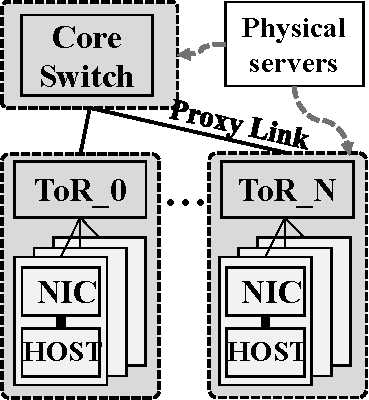
\includegraphics[width=0.8\linewidth]{figures/large_scale.pdf}
\vspace{8mm}
\caption{Large scale simulation configuration.}
\label{fig:largescale-config}
\end{minipage}%
\Description{Three subfigures: 9, 10, 11.

  The first subfigure (fig. 9) is a bar graph with PCIe latency on the
  x-axis and simulation time on the y-axis. As the latency increases
  from 1\,ns to 1000\,ns simulation time decreases from 117 minutes to
  about 72.

  The second subfigure (fig. 10) is a line graph comparing latency on
  the y-axis for end-host sequencer, switch-sequencer, and Multi-Paxos
  as throughput on the x-axis increases. The lowest line is the switch
  sequencer flat at around 40 microseconds starting at 20 thousand
  requests per second, until it hist saturation and rapidly increases
  at 75 thousand requests per second. The end-host sequencer
  configuration achieves a flat higher latency at around 55
  microseconds and saturates at the same point. Multi-Paxos already
  incurs 70 microseconds at 12 thousand requests, 90 microseconds at
  20 thousand requests, and then saturates.

  The third subfigure (fig. 11) is a diagram showing the large-scale
  simulation configuration, with boxes representing groups of
  simulators running on separate physical server. Each server contains
  a group of simulators and connects to one central server through
  proxy links. One server contains just one core switch. The remaining
  servers contain a top of rack switch, and multiple NIC-host
  simulators connecting to the top of rack switch. The Top of rack
  switch connects to the core switch through the proxy.}%
\end{figure*}


%%%%%%%%%%%%%%%%%%%%%%%%%%%%%%%%%%%%%%%%%%%%%%%%%%%%%%%%%%%%%%%%%%%%%%%%%%%%%%%
\subsubsection{Scaling Out}\hfill\\
%
We now move on to \sysname simulations running across
multiple physical hosts, using our RDMA and TCP proxies
(\autoref{fig:largescale-config}).

\paragraph{Overhead of distributed simulation.}
First we compare performance for local simulations to equivalent
distributed simulations with the \sysname proxies, to measure
overheads.
%
We use two qemu-kvm hosts running \texttt{netperf} connected to
\texttt{i40e} NICs which connect to the same switch.
%
Locally, this unsynchronized simulation yields a throughput of
4.4\,Gbps, and a latency of 71\,$\mu$s.
%
Next we distribute the simulation by running one pair of QEMU and NIC
on a second server and proxying the Ethernet connection to the switch
running locally.
%
With the sockets proxy the latency increases to 305\,$\mu$s and
throughput remains constant, and with RDMA both remain constant.
%
Next we measure simulation time for the same configuration but with
QEMU timing and gem5, and find that simulation time does not change
with either proxy.
%
We conclude that \emph{\sysname proxies are no bottleneck for
synchronized simulations.}

\paragraph{Large-scale memcache cluster.}
To evaluate scalability to larger systems, we next run multiple
distributed simulations ranging from 40 to 1000 simulated hosts, on 1
to 26 physical servers.
%
We run these simulations on Amazon ec2 \texttt{c5.metal} (spot)
instances, with 96 hyperthreads each, and 20\,Gbps network
connectivity in a single proximity placement group.
%
We simulate a varying number of racks of 40 hosts with \texttt{i40e}
NICs and a top of rack (ToR) switch each, that then connect to a
single core switch, as shown in \autoref{fig:largescale-config}.
%
We assign the core switch and each rack to a dedicated server.
%
A separate sockets proxy pair (Amazon ec2 does not offer RDMA)
connects each ToR to the core switch.
%
We run \texttt{memcached} on half of the hosts in each rack, and the
\texttt{memaslap} client on the other half.
%
Each client randomly connects to the 20 servers on the same rack, and
to 20 random servers in other racks.

\autoref{fig:large-scale} shows the measured simulation time for 10\,s
of virtual time as we increase the number of hosts.
%
From one rack and 40 hosts to 25 racks and 1000 hosts,
simulation time with gem5 hosts increases by 13.8\% from 15.5\,h,
to 17.6\,h.
%
With QEMU-timing, simulation time increases from 2.2\,h to 5.6\,h by
2.5$\times$.
%
With profiling we found the cause to be QEMU's dynamic binary
translation.
%
When an instance misses in its code cache and has to recompile a
block, the instance blocks for a while.
%
While rare, at scale these occurrences grow more frequent, and slow down
other hosts due to synchronization.
%
We conclude that \emph{\sysname scales to simulate systems with 100s
of hosts.}


%%%%%%%%%%%%%%%%%%%%%%%%%%%%%%%%%%%%%%%%%%%%%%%%%%%%%%%%%%%%%%%%%%%%%%%%%%%%%%%
\subsection{\sysname is Accurate}
\label{ssec:eval:accurate}
We now show \emph{\sysname Ethernet and PCIe interfaces accurately
connect and synchronize simulators}.
%
For Ethernet, we first run a pure ns-3 simulation of two communicating
nodes connected by a network link with our default parameters, and
log packet timestamps on each node.
%
Next, we repeat the experiment with two ns-3 instances each containing
one node and a \sysname Ethernet adapter, and connect the two.
%
For PCIe, we run two gem5 instances running netperf with the built-in
\texttt{e1000} NIC connected through the \sysname Ethernet adapter to a
switch.
%
We rerun this experiment with our standalone version of
gem5's \texttt{e1000} connected to both simulators through the \sysname
PCIe adapter.
%
In both cases we find that the timestamped logs match \textit{exactly},
demonstrating the correctness of our synchronization.


%%%%%%%%%%%%%%%%%%%%%%%%%%%%%%%%%%%%%%%%%%%%%%%%%%%%%%%%%%%%%%%%%%%%%%%%%%%%%%%
\subsection{\sysname is Deterministic}
\label{ssec:eval:deterministic}
Finally, we verify that \emph{\sysname simulations with deterministic component
simulators yields deterministic end-to-end simulations}.
%
To this end, we have repeated the two configurations combining only
deterministic simulators in \autoref{tab:modcombo} 5 times on
different machines.
%
We then compared event timestamps in the simulation logs and found
that they match \textit{exactly}.
